Figure~\ref{fig:4:fw} in Chapter~\ref{chap:cc.fw} shows the structure of the
congestion control framework described in this thesis. The framework
categorizes \emph{In-path} and \emph{Off-path} sources and \emph{out-of-band}
signaling for implementing congestion control (corresponds to
\emph{Block B and D} of Figure~\ref{fig:4:fw}). This chapter is based on our
work on network assisted congestion control, which is documented in
\citepub{c:3grc}, \citepub{c:glass} and \cite{glass:patent}.

In a 3G network, mobility, cell loading, handover and other factors can
affect the throughput available to each user and the varying network capacity
affects the video quality~\cite{diaz2007evaluating}. Deployments of GPRS, 3G
and LTE show that there are still geographical areas where capacity or
coverage is constrained~\cite{Curcio:glass, 6576402}. These constrained
geographical areas may occur due to fading and interference from large
building structures or closed or inaccessible areas (e.g., tunnels, boats on
lakes or in the archipelago, rural areas).

In \citepub{c:3grc}, when the available link capacity changes at a base
station, it notifies the endpoints connected to it about the current capacity.
Based on the notifications the sender adapts the media sending rate. Hence,
this paper covers the \emph{in-path} sources and \emph{out-of-band} signaling
of the framework defined in Chapter~\ref{chap:cc.fw}. We evaluate the
performance of employing network-assistance for congestion control in a
simulated environment using real-world 3G traces.

In \citepub{c:glass}, we explore the use of coverage maps for congestion
control. The map server collects throughput information from the mobile
clients, which also add geo-location information along with the throughput
information. This assists the map server to build a bandwidth and coverage
map. The server may be queried by mobile clients to predict coverage outage.
This paper covers the \emph{off-path} sources (e.g., coverage map)
signaling congestion cues \emph{out-of-band} to the endpoints. The paper also
discusses the protocol and implementation aspects of such a service. Lastly,
we evaluate the performance of using a coverage map for congestion control by
collecting 3G traces and emulating it in our testbed.

\section{In-path Congestion Cues}

% ECN, PCN, BW indication

In some network deployments, routers along the media path are capable of
detecting congestion before the queue overflows, typically, using active queue
management (e.g., RED). A router marks a packet, indicating that the packet
experienced congestion and the router would soon drop packets for this
flow~\cite{rfc3168}. The receiver on receiving this indication keeps a counter
for the number of ECN marked IP packets and signals it to the sender. For
performing congestion control, the sender typically treats the count of ECN
marked packets as lost packets~\cite{rfc6679}. For example, the sender uses
the sum of the reported loss events and the reported ECN events as the
\emph{p} (loss) value in the TFRC equation. Network-Assisted Dynamic
Adaptation (NADA)~\cite{rmcat-nada} propose a delay-based congestion control.
The receiver measures congestion by aggregating the packet loss count,
reported ECN markings, and one-way delay measurements into a single cue. The
sender calculates the new rate based on the variation in the delay cue
compared to earlier measurements and the priority of the multimedia
stream~\cite{pv-nada}.

\begin{figure}
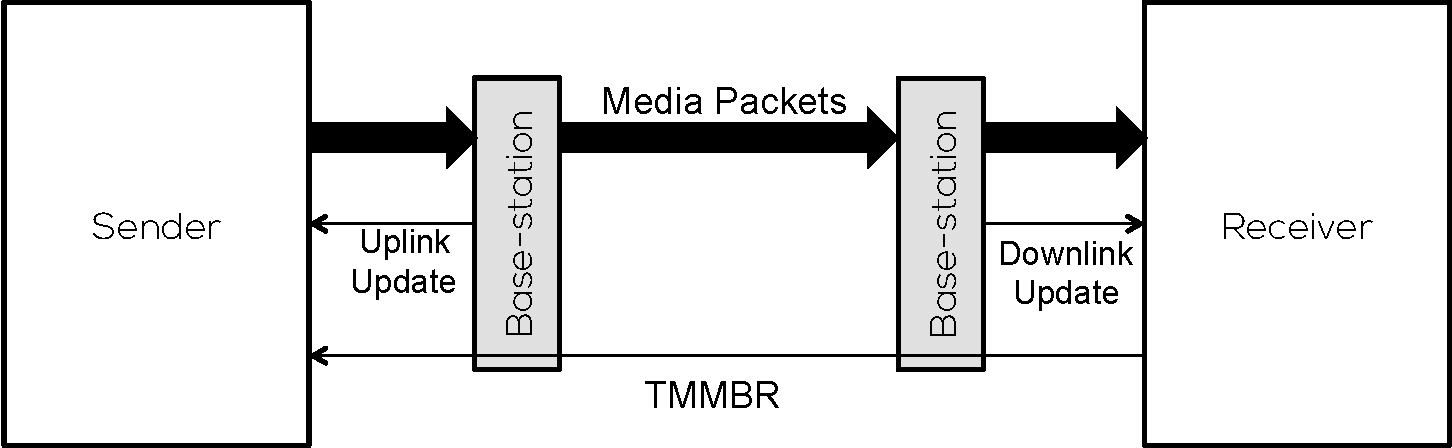
\includegraphics[width=\textwidth]{chap8-fig-tmmbr}
  \caption{Endpoints receiving capacity indication from the middleboxes
  (TMMBR) for implementing congestion control.}
\label{fig:cc:tmmbrab}
\end{figure}

In wireless networks, such as 3G/LTE, the last hop is typically the bottleneck
because the core network is well provisioned. In \citepub{c:3grc}, we
implement a network-assisted congestion control scheme, wherein base-stations
(along the media path) notify the mobile terminals about the available link
capacity. In TMMBR-A, the base-stations notify both the sending and receiving
endpoints about the available capacity, i.e., the sender is notified about the
uplink capacity and the receiver is notified about the downlink capacity. If
an endpoint sends and receives data, it is notified asynchronously about the
uplink and downlink capacity. Figure~\ref{fig:cc:tmmbrab} shows a schematic
representation about the interaction between the middleboxes and the
endpoints. In TMMBR-B, the receiving endpoint is solely notified about the
downlink capacity. Both TMMBR-A and TMMBR-B employ a co-operative congestion
control scheme, wherein the receiver sends a TMMBR request to the sender
containing the current downlink capacity. In TMMBR-A the sender also receives
a notification about the uplink capacity from the base-station, hence,
comparing the request from the receiver and the notification from the base-station, 
it chooses the minimum of the two values as the new sending rate. In
TMMBR-B, the sender calculates the \emph{sender's estimate} (similar to the
one described in~\ref{cc:co-op}) and chooses the minimum of the sender's
estimate and the receiver's bit rate request. 


Figure~\ref{fig:tmmbn} shows the sample performance of TMMBR-A and TMMBR-B,
where both endpoints are sending media over a 3G network. TMMBR-A due to its
knowledge about the network conditions at the uplink and the downlink provides
an average througput of 180\,kbps and 0\% loss, while TMMBR-B provides
comparable throughput 178\,kbps but with a 2\% loss ratio.

% Eventhough modern 3G/LTE networks are capable of providing these updates, they
% do not for several reasons

\begin{figure}
  \centerline{
    \subfloat[TMMBR-A]{
      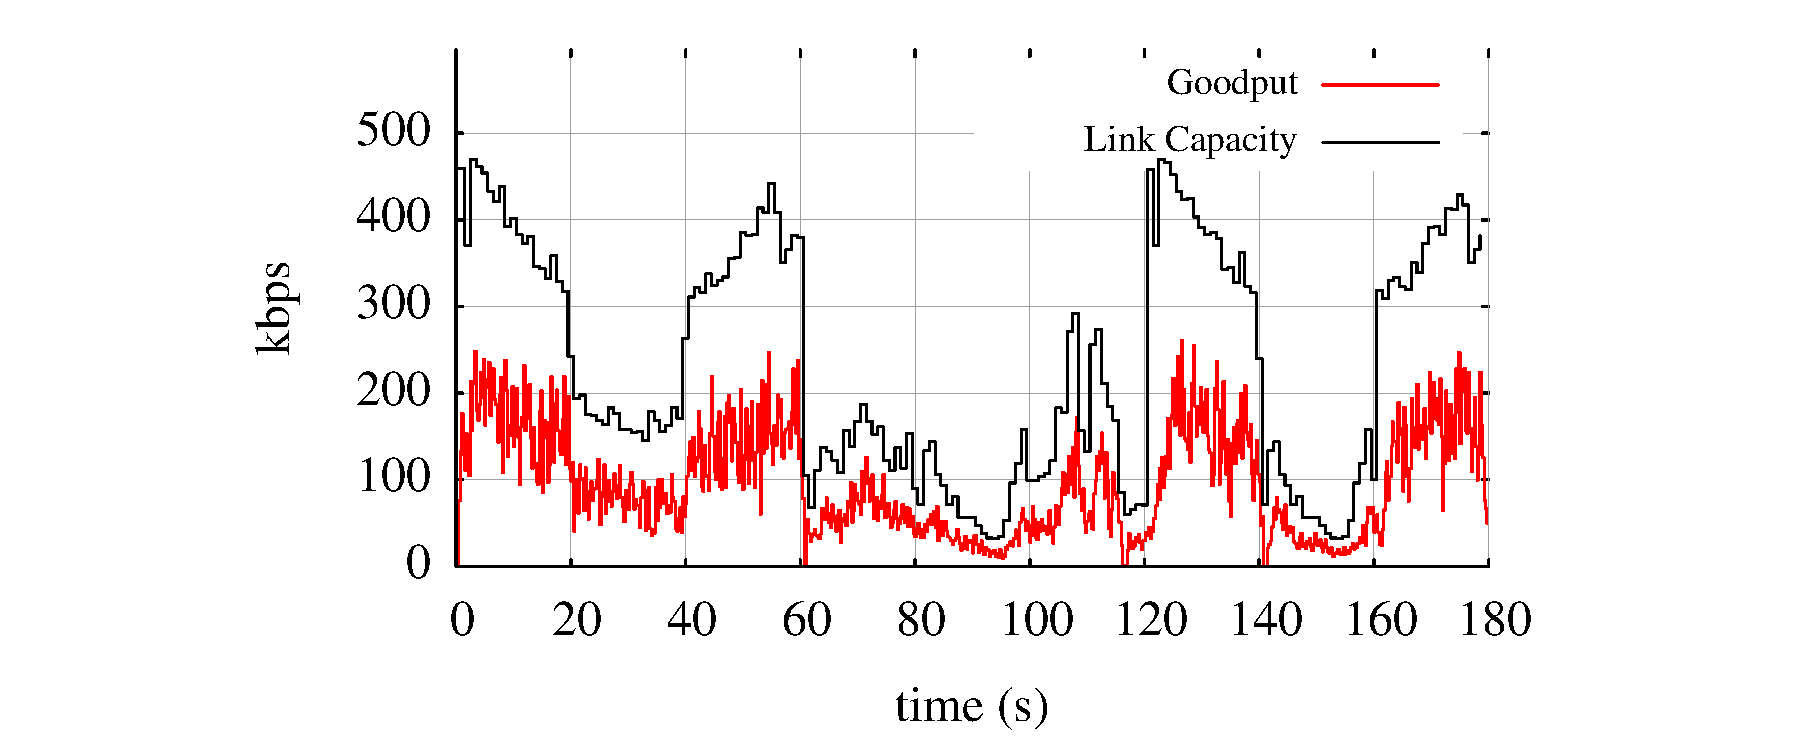
\includegraphics[width=0.5\textwidth, clip=true, trim=3cm 0 4.5cm 0]
      {chap8_graph_3g_tmmbr_a}
    }
    \subfloat[TMMBR-B]{
      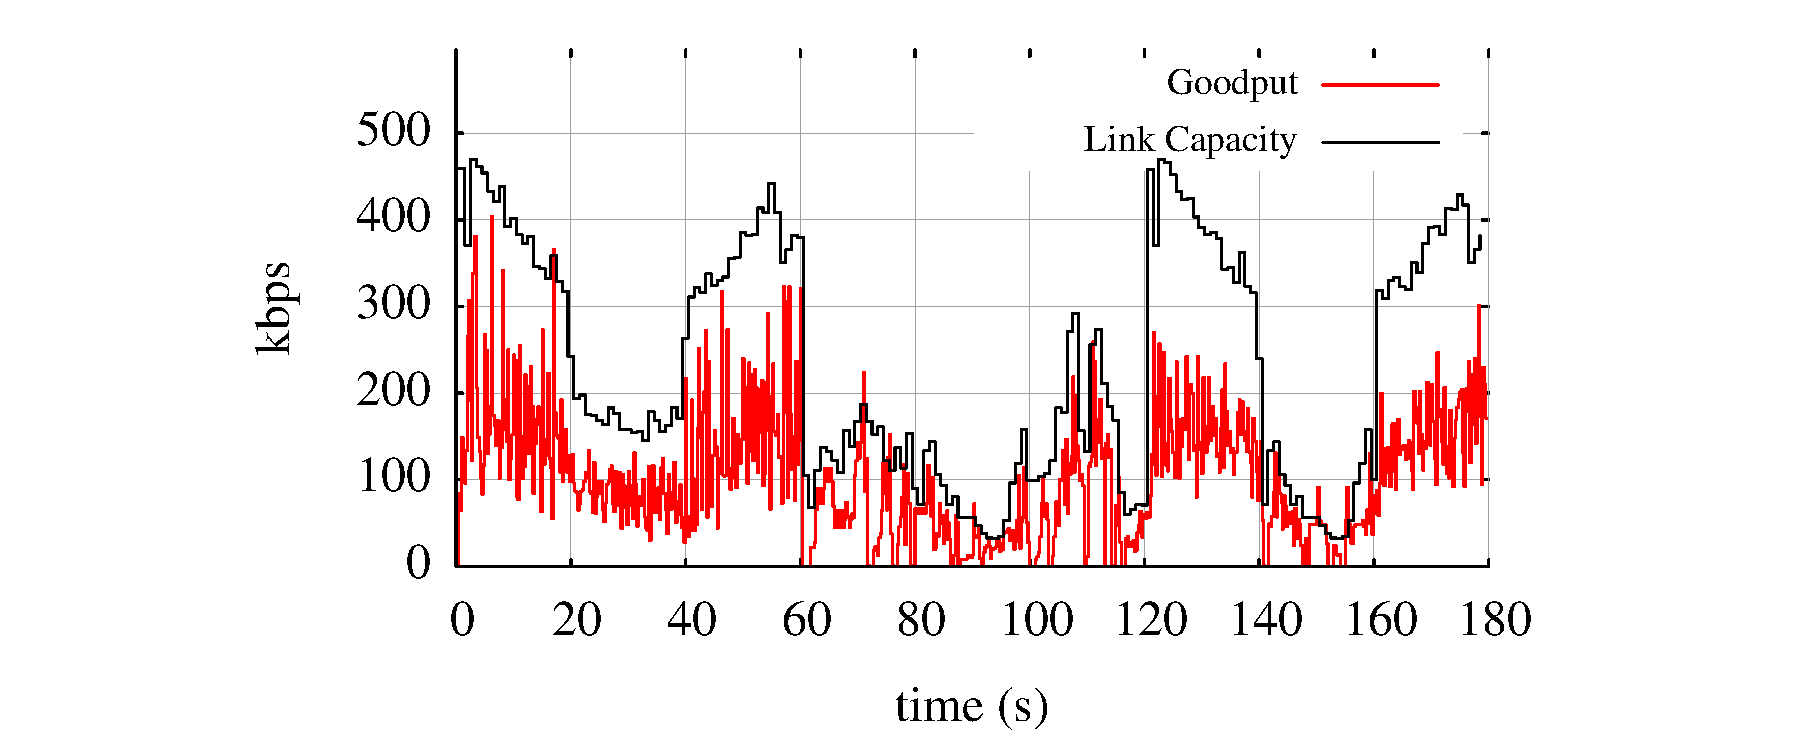
\includegraphics[width=0.5\textwidth, clip=true, trim=3cm 0 4.5cm 0]
      {chap8_graph_3g_tmmbr_b}
    }
  }
  \caption{The plots show the performance of bandwidth indications by the base
  stations a) TMMBR-A: both terminals are assisted, b) TMMBR-B: the receiver
  is only assisted.}
  \label{fig:tmmbn}
\end{figure}


\section{Off-path Congestion Cues}

% Congestion map

Modern mobile networks have been designed to carry multimedia streams with QoS
traffic classes~\cite{3gpp.23.107}, but deployments of GPRS, 3G and HSDPA
networks show that there are still geographical areas where best-effort
traffic classes are used~\cite{Curcio:glass, 6012045}. These constrained
geographical may occur due to fading and interference from large building
structures or closed or inaccessible areas (e.g., tunnels, boats on lakes or
in the archipelago, rural areas). To overcome these challenges, in
\citepub{c:glass}, we implement a bandwidth coverage map that collects
connectivity information from the users (\emph {crowd-sourcing}) and
calculates the available capacity at the reported geographical locations.

Service Maps are presented in~\cite{1630563} and the measurement based
approach is proposed in~\cite{Aravinda:2008p14}. GPS-based congestion control
is introduced in~\cite{Yao:2008p21}, and evaluated in different
scenarios~\cite{Yao:2009p57}, \cite{Yao:2010p64}, but they take signal
strength as an influential factor for rate-control and show that predicting
based on signal strength alone is insufficient. Yet, their results indicate
that past information can be used to predict future network characteristics.

\cite{6012045} proposes a similar architecture (\emph{bandwidth lookup
service}) to the one in \citepub{c:glass}, but uses different types of
averaging algorithms to predict future network characteristics in Dynamic
Adaptive Streaming over HTTP (DASH). While the averaging algorithm is not a
focus of this thesis, we use K-means~\cite{Kanungo:2002:LSA:513400.513402} and
K-nearest neighbor (K-NN)~\cite{Iwerks:2003:CKN:1315451.1315496} algorithms to
form regions with similar bandwidth. Details of the averaging algorithms
employed by our coverage map server are discussed in~\cite{sharmistha-thesis}.
A contrary approach is employed by \emph{Netradar.org}~\cite{6576402}, which
divides the geographic map into 100m\,x\,100m squares, all measurements in a
specific area are averaged. Additionally, \cite{Riiser:2012:2240136} proposes
fetching the bandwidth along a travel route in steps of 100 meters, which we
find limiting. Instead we propose multiple methods for discovering areas with
poor connectivity (e.g., known travel route, area look ahead, geo-fencing or
subscribing to coverage holes.) and show that not only looking up future
bandwidth but also when to vary the sending rate affects the usefulness of the
service. A preliminary analysis using simulations of our system is done
in~\cite{Curcio:glass}.

\begin{figure}
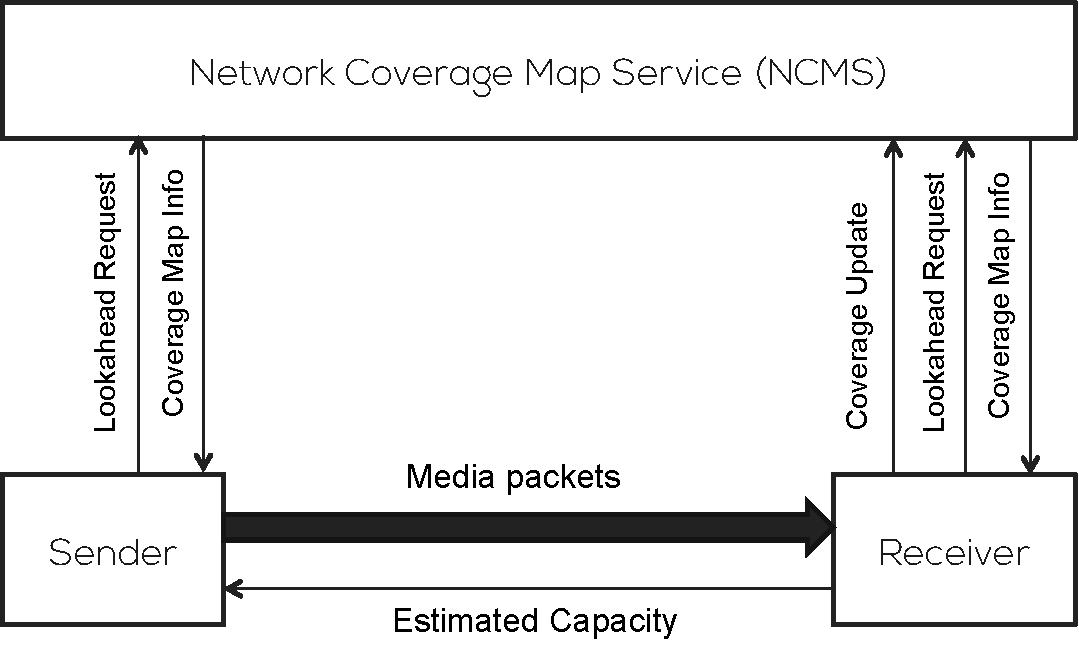
\includegraphics[width=\textwidth]{chap8-fig-ecv}
  \caption{Endpoints using a Network Coverage Map Service to send coverage
  updates, query for upcoming congestion and receive coverage updates.}
\label{fig:cc:ecv}
\end{figure}

\begin{figure}
  \centerline{
    \subfloat[Map Area Lookahead]{
      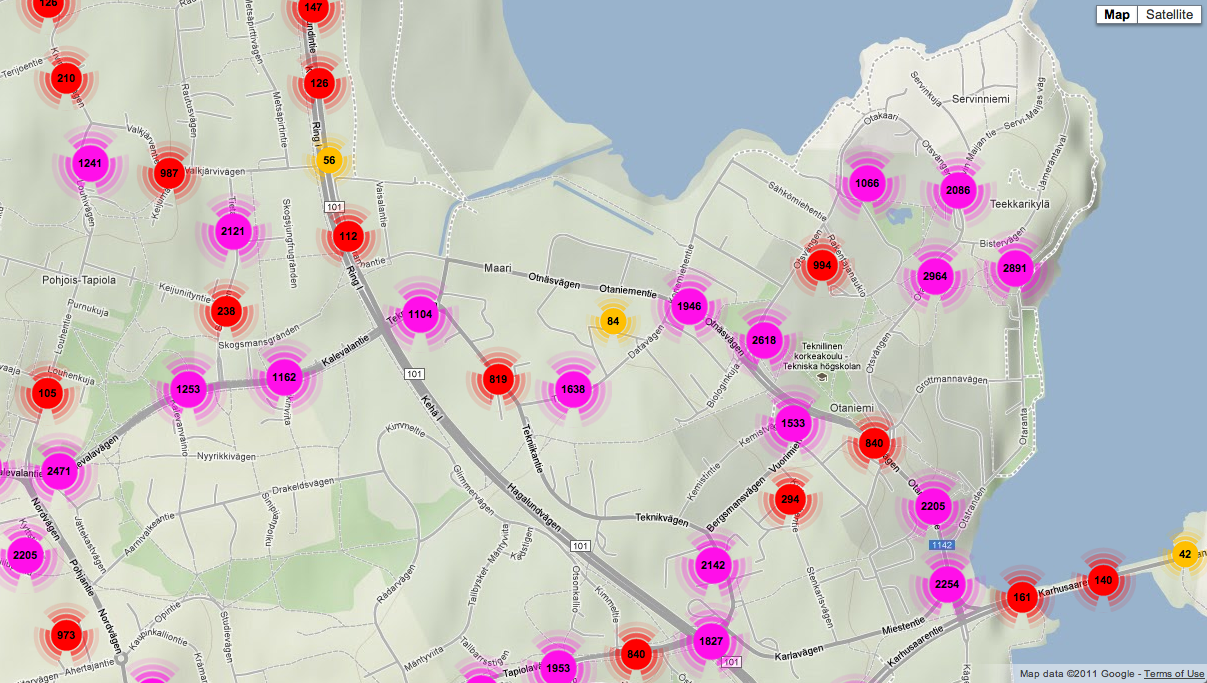
\includegraphics[width=0.8\textwidth]
      {chap8-fig-ota-tr-net-02}
    }
  }
  \centerline{
    \subfloat[Known Travel Route Lookahead]{
      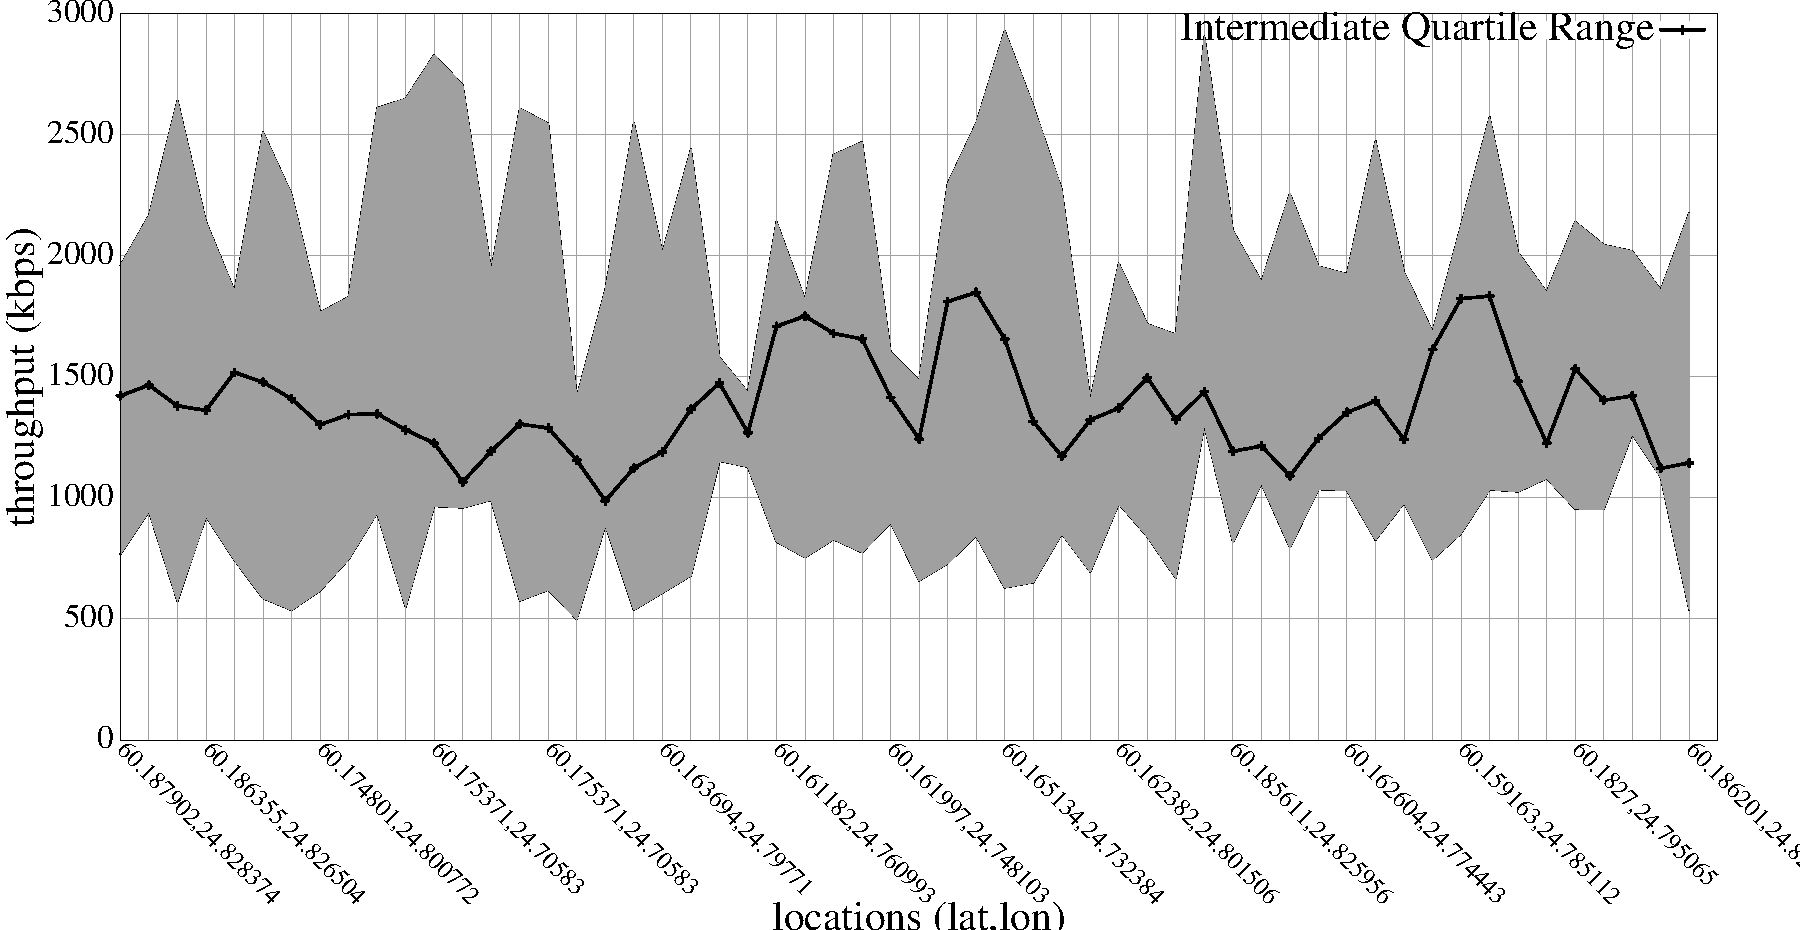
\includegraphics[width=0.8\textwidth]
      {chap8-graph_route_thin_throughput}
    }
  }
  \caption{a) A map of the available capacity around Otaniemi (university
  area). b) Example of the average and the Inter Quartile Range
  ($IQR=\pm1\sigma$) throughput along a known route. The data in both
  representations are captured over several days.}
  \label{fig:glass:map}
\end{figure}

In \citepub{c:glass}, we present a mechanism enabling an endpoint (usually a
receiver) to proactively react to upcoming capacity limitations in wireless
access networks. We enable this by implementing three steps,
Figure~\ref{fig:cc:ecv} shows the interaction between the endpoints and the
Network Coverage Map Server (NCMS). First, each endpoint receiving a media
stream monitors the throughput and its geolocation and reports it to the NCMS.
Figure~\ref{fig:glass:map} shows the throughput around the university area in
Espoo. Second, each endpoint is capable of querying the NCMS for upcoming
congestion (known as \emph{lookahead}). It can \emph{lookahead} using one of
the following methods: known travel route, area lookahead or by subscribing to
areas with poor coverage, typically using geo-fencing\footnote{Areas where the
expected channel capacity is lower than the media bit rate}.
Figure~\ref{fig:glass:map} shows a graphical representation of the average
throughput for a \emph{area lookahead} and a \emph{known travel route}. Third,
for each lookahead requests, the NCMS responds with an coverage map info,
i.e., the expected throughput at every geolocation along the route or
requested area.

The receiver uses these hints provided by the NCMS to implement congestion
control and sends an \emph{estimated capacity vector} (a data structure
containing a time-series of available throughput, thus preserving user's
location privacy) to the sender, which can alter the sending rate based on the
received information. The sender has the following techniques to change the
sending rate: 1) adapt the encoding rate, 2) perform a rate-switch, or, 3)
pre-buffer. Changing the encoding rate is only possible in interactive 
real-time media, because the RTP sender co-operates with the encoder to  modify the
encoding rate. Rate-switching is possible for streaming content  encoded at
different bit rates. It is also possible to use rate-switching  for
interactive real-time media involving scalable video codecs or simulcast
media, wherein a media stream is encoded at different bit rates and the
application switches between the stored media files. The performance of the
congestion control in this case depends on the granularity of the chosen bit
rates for the individual media streams. Lastly, varying the amount of 
pre-buffered video provides a more consistent experience to the user,  because the
technique attempts to maintain multimedia play back at a constant  media
encoding rate. It is only applicable to stored content, the application,
typically, reads-ahead in the media stream and sends more data whenever before
it detects poor coverage.

In \citepub{c:glass}, video is sent from a server to mobile clients. The user
in the experiments mainly commute around the city of Helsinki and Espoo using
public transport. The NCMS collects the measured throughput for each client,
thereafter, we conduct simulated experiments of users traveling at different
vehicular speeds through the Helsinki region. In total, the NCMS collected
over 400,000 updates over a month of operation (about 40-50 bus-trips). The
NCMS received more than 10,000 updates for 6 geographical areas
(\emph{Otaniemi}, Helsinki City Center) while on average each geographical
location had around 100 updates.

In \citepub{c:glass} we describe a scenario where a user moves smoothly
through a set of locations along a route and the receiver performs
\emph{lookahead} queries to fetch coverage information for surrounding areas.
In this scenario, there are gaps in coverage but overall the throughput at
most locations is above the required media rate. We analyse the performance of
4 different algorithms, they are: 1) the \emph{omniscient algorithm}, the
endpoint is aware of the exact end-to-end channel capacity and is expected to
perform the perfect rate-adaptation. 2) \emph{no adaptation}, the endpoints
perform no congestion control and the stream is transmitted at a constant bit
rate. In the periods when the link capacity falls below the media rate, the 
receiver will observe an increase in losses/discards, which may result in 
frequent pausing of the video. 3) \emph{Rate-switching}, the endpoints perform short
\emph{lookaheads}, which enables the endpoints to detect outages a few moments
before the user enters a location with poor connectivity. In this case, the
receiver sends a TMMBR message (with lowest available bit rate in the area)
before entering the area and another one after the exiting the area (to reset
the bit rate). The sender reacts by switching the media stream to the closest
available media rate. 4) \emph{Late scheduling}, the receiving endpoint
searches for areas with poor coverage much before the user arrives at those
locations, so that it can pre-buffer the content equivalent to the duration of
the disruption. To reduce the impact of changing routes, the streaming client
uses the congestion control algorithm proposed in \citepub{c:glass}.

\begin{table}
  \begin{center}
\begin{tabular}{ccccccc} \hline
Method & $SR_{avg}$ & $PSNR_{avg}$ & $\sigma_{PSNR}$ & PLR \\ \hline
% & $buffer_{max}$\\ \hline
No adaptation   & 865   & 27.48 & 4.55  & 6.6 \\
Omniscient      & 929   & 43.12 & 1.9   & 0.33 \\ 
Rate-switching  & 881   & 42.75 & 2.21  & 0.0  \\ 
Late scheduling & 1014  & 48.43 & 0.18 & 0.0  \\ \hline
\end{tabular}
\caption{A bus ride with good 3G coverage.}
\label{table-glass-sim7res}
\end{center}
\end{table}


Table~\ref{table-glass-sim7res} compares the results for the different schemes
and Figure~\ref{fig:glass:sim7res} shows the sending/receiver rate variation
to channel throughput for one out of 10 simulation runs. The \emph{omniscient
algorithm}  provides the best rate-adaptation but since it is unable to 
pre-buffer, the PSNR ($PSNR_{avg}$=43) is lower than that of late scheduling
($PSNR_{avg}$=48). Alternatively, performing \emph{no adaptation} causes
frequent pausing when the capacity is lower than the media rate, additionally
packet loss too affects the media quality and is reflected in the low PSNR
($PSNR_{avg}$=27). \emph{Rate-switching} has comparable results to the
\emph{omniscient} case because it avoids congestion by switching to bit rates
lower than the minimum reported throughput. There are no losses  and average
PSNR is 42.75, which is comparable to the \emph{omniscient} case. \emph{Late
scheduling} outperforms the rest of the schemes in terms of media quality
(measured in terms of average PSNR, $PSNR_{avg}$=48.43) mainly because it
attempts to stream media at a single quality level, it relies heavily on 
pre-buffering, constantly updating the size of the pre-buffer to compensate for
the longest disruption it finds along the travel-route or in the viscinity of
the user. Another reason is that in our measurements we found low density of
poor coverage areas and good connectivity in areas in between allowing the
client to pre-buffer content. However, when it is not possible to pre-buffer,
the client will perform a rate-switch. Finally, we expect the performance of
the congestion control to be at least that of rate-switching because the
sender will be able to vary the sending rate preemptively without probing.

\begin{figure}
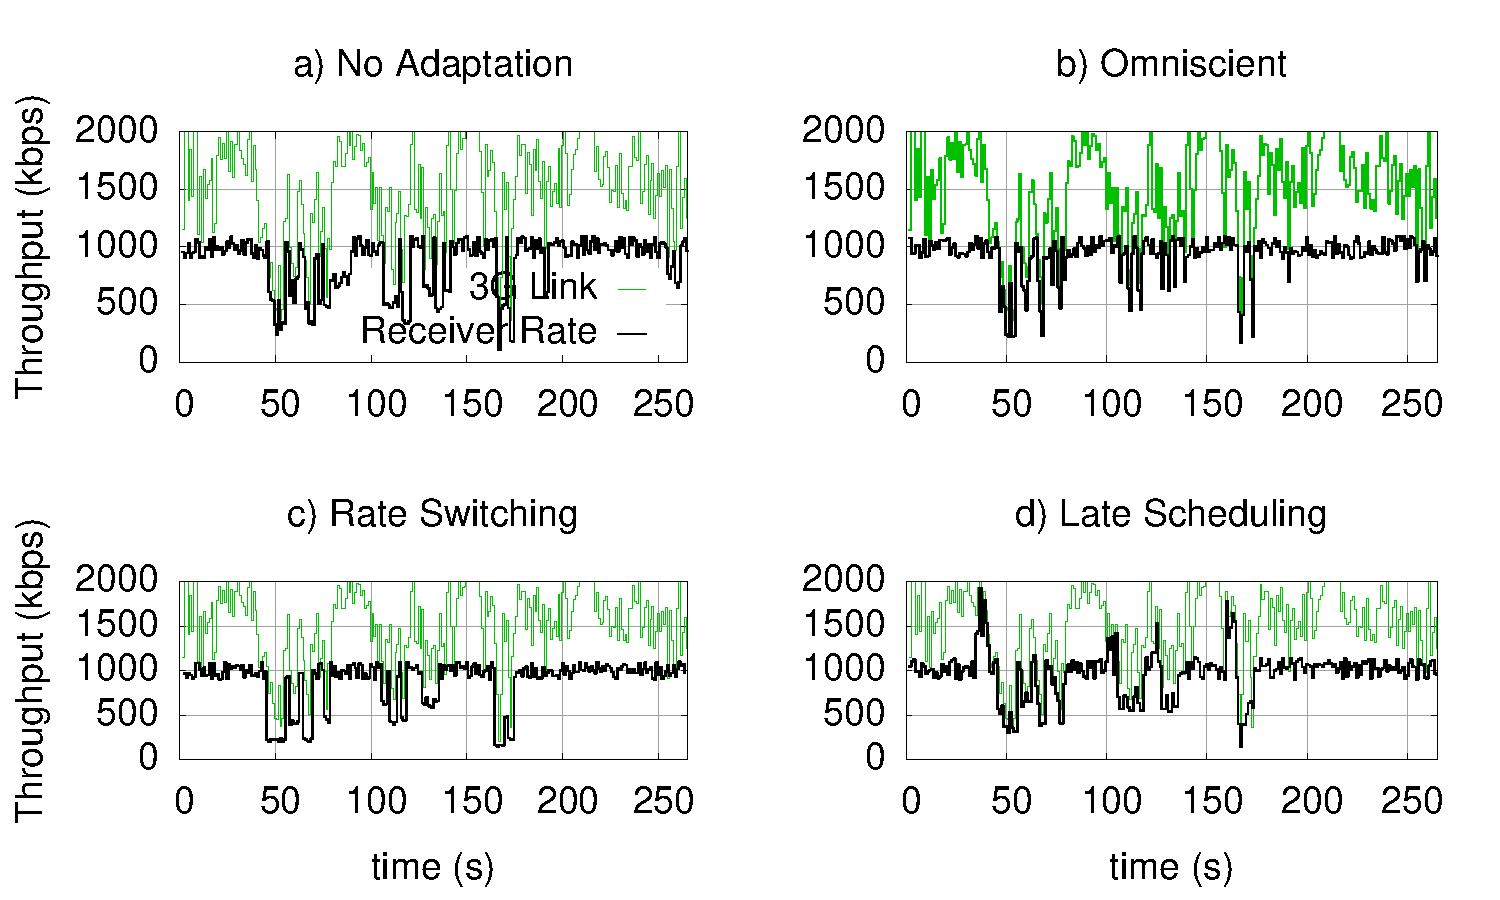
\includegraphics[width=\textwidth]{chap8-graph-sim7-3}
  \caption{The plot shows the variation of sending rate to 3G link capacity
  based on a) no adaptation b) Omniscient c) Rate-switching d) Late scheduling
  when there are few coverage holes and good connectivity between them.}
\label{fig:glass:sim7res}
\end{figure}


We find that the information provided by the NCMS is suitable for both
predictive rate-switching and  pre-buffering and helped in avoiding almost all
packet losses in the scenarios we investigated, noticeably increasing video
quality. This system wprks for video streaming and can be adapted for
interactive media communication, wherein the sender employs a co-operative
congestion control scheme, i.e., the sender receives the \emph{estimated
capacity vector} from the receiver and \emph{coverage map information} for
itself from the NCMS, it then picks the minimum of the two rates and any
additional rate recommended by the congestion control (one of the algorithms
discussed in Chapter~\ref{chap:cc}) it implements.

\section{Summary}

In this chapter we describe two congestion control mechanisms, both  use out-
of-band signaling, but use in-path and off-path sources, respectively. First,
the in-path sources is based on receiving congestion cues from middleboxes
(e.g., 3G or LTE base-stations) and use standard RTP extensions (e.g., TMMBR)
for signaling . Second, the off-path source is a crowd-sourced 3G coverage
map that collect throughput and geo-location information from users and then
notifies the subscribed endpoints about the available capacity in their
respective neighborhoods. We propose a system to collect and query coverage
maps. The endpoints query the coverage server using out-of-band signaling to
discover areas of poor coverage, based on these notifications the endpoints
vary their sending rate.

We show that notification from middleboxes such as, by base stations would
help endpoints better congestion control for example in mobile networks, for
example when an LTE cell is experiencing extreme load\footnote{Extreme load
occurs when an LTE cell has about 10x more users than when it is busy.}.
Furthermore, we also show that using congestion maps also aids in performing
congestion control. Congestion maps is a measurement service that aggregates
throughput information from multiple users and sends notification of areas
with poor coverage to its subscribers. We expect these notifications to be
used as congestion cues and not as a replacement to in-band, in-path
congestion control. The main reason for restricting the use of such a service
to notify congestion cues is that such a service is vulnerable to data
pollution, i.e., the clients may report incorrect measurements, not
necessarily intentionally but because of programming errors. Another reason is
that the reported notifications may depend on the way the aggregation is
performed and how quickly the aggregation converges to the prevailing network
conditions in a region. A fast convergence may be susceptible to misreporting
leading to false positives and make the user experience fluctuate when in
reality there would be no reason for it to fluctuate. A slow convergence would
ignore minor spikes in load and endpoints would experience poor quality of
experience for a brief period until the values converge. A slow convergence
may also lead to inefficiency because once an aggregation value in a region
drops; it would stay there unless the endpoints probe for additional capacity.

While we show that NCMS can be used for streaming both the live and stored
multimedia content, it can be adapted to work with interactive media services.
However, we believe that the NCMS notifications would perform best when
working alongside an exisiting congestion control algorithm.
